\documentclass[12pt]{article}

\usepackage{graphicx}
\usepackage{tikz}

\title{AMath Tea Time --- Puzzle \#4}
\author{}
\date{\vspace{-1cm}21 April 2015}

\begin{document}

\maketitle
\pagenumbering{gobble}

\subsection*{Problem}

An infinite number of lilypads grow in a line, numbered $\ldots, -2, -1, 0, 1,
2, \ldots$. Thumbelina and her pet frog start on one of the lilypads. She wants
to make a sequence of jumps that will end on either pad 0 or pad 96. On each
jump, Thumbelina tells her frog the distance (number of pads) to leap, but the
frog chooses whether to jump left or right. From which starting pads can she
always get to pad 0 or pad 96, regardless of her frog's decisions?

\begin{figure}[hb]
  \centering
  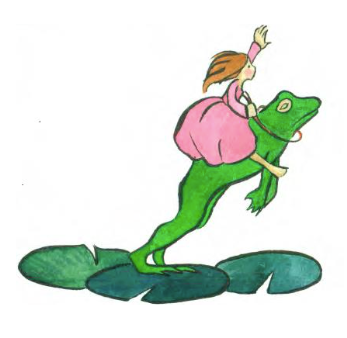
\includegraphics[width=120px]{thumb.png}
\end{figure}

\subsection*{Hints}

{\it (Posted on Thursday)}


{
\par\vspace*{\fill}
\noindent \small \it
If you have any puzzles to share then send them my way at {\tt
  cswiercz@uw.edu}!
}

\end{document}
